\chapter{Metodologia de Trabalho}
\label{chap:Metodo}

Neste capítulo é apresentado o método utilizado para o desenvolvimento deste trabalho. Foram envolvidos dois procedimentos de pesquisa científica e uma técnica de modelagem de design sobre as informações coletadas na pesquisa científica (Figura \ref{Fig:geral_flow.png}).

\begin{figure}[htbp]
	\centering
	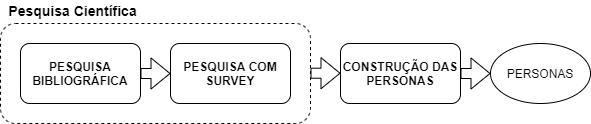
\includegraphics[keepaspectratio=true,scale=0.6]{figuras/metodologia/fluxo geral.png}
	\caption{Processo Metodológico do Trabalho - Autoral}
	\label{Fig:geral_flow.png}
\end{figure}

As metodologias apresentadas na Figura \ref{Fig:geral_flow.png} seguem descritas nas seções a seguir. A Seção \ref{sec:pesq_cient} apresenta a metodologia de pesquisa bibliográfica e da pesquisa com \textit{survey} e a Seção \ref{sec:const_person} descreve o processo de construção das personas. 


\section{Pesquisa Científica} 
\label{sec:pesq_cient}

Segundo \citeonline[p. 34-42]{Gerhardt2009}, a pequisa bibliográfica deste trabalho tem uma abordagem qualitativa, de natureza aplicada, com objetivo descritivo em relação aos conceitos sobre as personas, o método de criá-las e sobre as características de jogos para aprendizagem.

Esta pesquisa foi realizada de forma não sistemática, na qual foram selecionadas bases teórica \cite{barbosa_silva, BarbosaEtAl2021, cooper07} recomendadas pelos orientadores deste trabalho, a literatura utilizada no projeto de pesquisa Recursos Digitais Didáticos para Interação Humano-Computador\footnote{Repositório do projeto: \url{https://github.com/RecursosDigitaisdeEnsinoAprendizagemIHC}} (RDDIHC), artigos científicos publicados \cite{deSales_SousaeSilva_2020, silva_sales_mendes2021} e referências encontradas a partir da leitura destes. A interpretação e análise crítica das informações apresentadas na literatura adotada foram feitas pelo próprio autor deste trabalho \cite{ROTHER2007}. 
% O Capítulo \ref{chap:ref} apresenta o resultado dessa pesquisa bibliográfica. 

Na sequência foi realizada uma pesquisa com \textit{survey}. Alguns trabalhos estudados \cite{Petri_Wangenheim_2019, deSales_SousaeSilva_2020} na pesquisa bibliográfica serviram de base para esta pesquisa. O objetivo do \textit{survey} foi definir o público-alvo do jogo e identificar requisitos que atendessem a estes público de jogadores. Segundo \citeonline{Gerhardt2009}, a abordagem desta pesquisa é quali-quantitativo, de natureza aplicada, com objetivo descritivo utilizando-se de um questionário auto-aplicável para a realização da pesquisa com \textit{survey}. 

De acordo com \citeonline{Kasunic_2005} um \textit{survey} envolve a coleta e análise de dados na qual os entrevistados respondem a um instrumento de pesquisa previamente planejado. Um \textit{survey} consiste na execução de sete etapas, como apresentado na Figura \ref{Fig:survey_flow.png}.

\begin{figure}[htbp]
	\centering
	\caption{Processo de Pesquisa com Survey}
	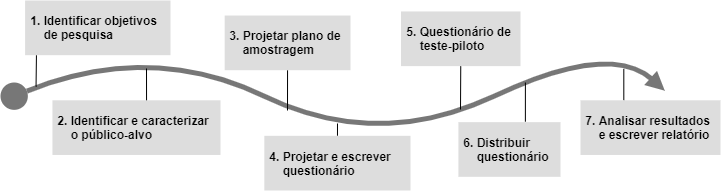
\includegraphics[keepaspectratio=true,scale=0.55]{figuras/metodologia/flow_survey.png}
	\legend{Fonte: Traduzido de \citeonline{Kasunic_2005}}
	\label{Fig:survey_flow.png}
\end{figure}

O processo se inicia com a identificação do objetivo de pesquisa como é apresentado na primeira etapa da Figura \ref{Fig:survey_flow.png}. Os objetivos foram definidos como ``caracterizar os usuários de jogos para aprendizagem'' e ``identificar a relevância dos aspectos de qualidade em jogos sérios para aprendizagem''. 

Seguindo o fluxo na Figura \ref{Fig:survey_flow.png}, na segunda etapa, identificação e caracterização do público-alvo, foi adotado nesta pesquisa a população de alunos de graduação e pós-graduação de cursos da área de Ciência da Computação. 

A terceira etapa da Figura \ref{Fig:survey_flow.png} aborda a realização do plano de amostragem, que foi definido no presente trabalho para ser realizado em instituições de ensino de graduação e pós-graduação. A coleta dos dados foi planejada para ser executada via questionário virtual, no período entre os dias 06/10/2020 e 27/10/2020. 

As perguntas elaboradas para o questionário, na quarta etapa (Figura \ref{Fig:survey_flow.png}), buscaram identificar os atributos do modelo de personas apresentado em \citeauthor{usability2020} e por \citeonline{BarbosaEtAl2021}, além das características de jogos sérios em IHC identificados por \citeonline{deSales_SousaeSilva_2020} e das metas de usabilidade e experiências do jogador descritas por \citeonline{Petri_Wangenheim_2019}.

O questionário passou por rodadas de teste, correções e melhorias, como prescreve a quinta etapa (Figura \ref{Fig:survey_flow.png}), além de detectar quaisquer outros erros e contabilizar o tempo médio para se realizar o questionário. O teste também verificou se as questões estavam fáceis de serem entendidas e se o \textit{layout} e fluxo estavam adequados.

Na sequência, na sexta etapa (Figura \ref{Fig:survey_flow.png}), o questionário (Apêndice \ref{ap:questionario}) foi distribuído via mensagem eletrônica e redes sociais para a comunidade discente da Universidade Católica de Salvador (UCSAL), Universidade de Brasília (UnB), Universidade Federal de Uberlândia (UFU), Universidade Federal do Amazonas (UFAM),  Universidade Federal do Mato Grosso (UFMT), Universidade Federal do Mato Grosso do Sul (UFMS) e Universidade Tecnológica Federal do Paraná (UTFPR).

Na última etapa, conforme a Figura \ref{Fig:survey_flow.png}, os dados coletados foram armazenados em uma planilha eletrônica e ali analisados. Foram obtidas 184 respostas, porém com inconsistências em algumas delas. Das inconsistências, 8 pessoas responderam o questionário mais de uma vez e 10 respondentes não cursaram graduação na área de computação. Essas dezoito respostas foram removidas, restando portanto, um total de 166 respostas válidas. 

A análise dos dados, o procedimento, o questionário e os dados coletados, encontram-se no pacote de pesquisa do projeto\footnote{\url{https://github.com/RecursosDigitaisdeEnsinoAprendizagemIHC/research-pack-hci-games}}. Esta análise que se inicia na pesquisa com \textit{survey} e se estende para o processo de construção das personas. Na Seção \ref{sec:const_person} é apresentado este processo de construção das personas.

\section{Construção das Personas}
\label{sec:const_person}

O processo de construção das personas descrito por \citeonline{cooper07} apresenta sete etapas para definir um elenco de personas. Neste trabalho estas etapas foram executadas em três fases. A Figura \ref{Fig:construct_persona.png} demonstra uma visão geral do processo.

\begin{figure}[htbp]
	\centering
	\caption{Processo de Construção das personas}
	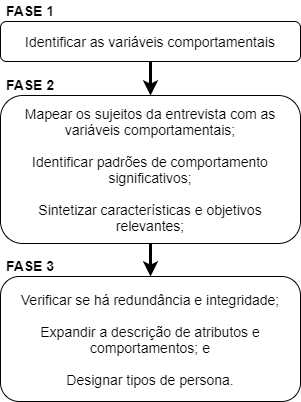
\includegraphics[keepaspectratio=true,scale=0.65]{figuras/metodologia/construct_persona.png}
	\legend{Fonte: Autoral}
	\label{Fig:construct_persona.png}
\end{figure}


As respostas de cada indivíduo foram registradas na planilha eletrônica (PE0). Este conjunto de dados foi o ponto de partida para a modelagem das personas.

Na primeira fase foram identificadas as variáveis comportamentais. Estas foram definidas a partir das perguntas do questionário. De acordo com as respostas dadas pelos respondentes foi-se agrupando os registros de respostas dos indivíduos que tinham características comportamentais semelhantes. Na Tabela \ref{tab:Table_variaveis-comp} estão as variáveis comportamentais identificadas, além das variáveis demográficas que foram coletadas dos respondentes. 

\begin{table}[htbp]
\centering
\caption{Variáveis Comportamentais}
\label{tab:Table_variaveis-comp}
\begin{tabular}{|p{4.7cm}|p{10cm}|}
\hline
\textbf{Questão} & \textbf{Variáveis}                             \\ \hline
O01   &  Relação com a Disciplina de IHC                          \\ \hline
H01   &  Experiência com design de interfaces                      \\ \hline
RL01   &  Ação para sanar dúvidas de algum conteúdo               \\ \hline
O02  &  Uso de jogos para aprender                \\ \hline
O02.1.1, O02.2.1, O02.3.1   &  Motivos para usar jogos para aprendizagem\\ \hline
O02.1.2, O02.2.2   &  Frequência no uso de jogos para aprendizagem\\ \hline
O02.1.4  & Motivos para deixar de usar jogos para aprendizagem       \\ \hline
O02.3.2  &  Motivos de nunca ter usado jogos para aprendizagem    \\ \hline
O02.4.1  & Motivos de não ter interesse em jogos para aprendizagem       \\ \hline
RE01  & Relevância dos fatores de usabilidade do jogo          \\ \hline
E01   & Importância dos fatores de experiência do jogo        \\ \hline
\end{tabular}
\legend{Fonte: Autor}
\end{table}

A Tabela \ref{tab:Table_variaveis-comp} relaciona o identificador de uma questão do questionário de pesquisa (terceira coluna) com suas respectivas variáveis (primeira coluna). Ainda nesta tabela são classificadas outros tipos de variáveis que não são consideradas comportamentais, mas que serviram no processo de modelagem das personas. As perguntas utilizadas para levantar essas variáveis encontram-se na Tabela \ref{tab:quest-survey}.  

Após a identificação das variáveis comportamentais seguiu-se para segunda fase, como é apresentado na Figura \ref{Fig:construct_persona.png}. Os passos foram o mapeamento dos respondentes em relação a essas variáveis, a identificação de padrões de comportamento significativos e a sintetização de características e objetivos relevantes.

Fez-se uso da planilha eletrônica (PE0) e suas ferramentas para a auxiliar o processo de filtragem e síntese dos dados. Primeiramente foram divididos em dois, os dados dos respondentes, a partir da variável I04. Assim foi definida as primeiras características da anti-persona (aqueles que não são da área de Ciência da Computação) e a estrutura base das demais personas (PE1), aqueles que da área da Ciência da Computação. Na Figura \ref{Fig:persona_tree.png} é apresentada o processo de refino dos dados para construção das personas.

\begin{figure}[htbp]
	\centering
	\caption{Fluxo do processo de construção das personas}
	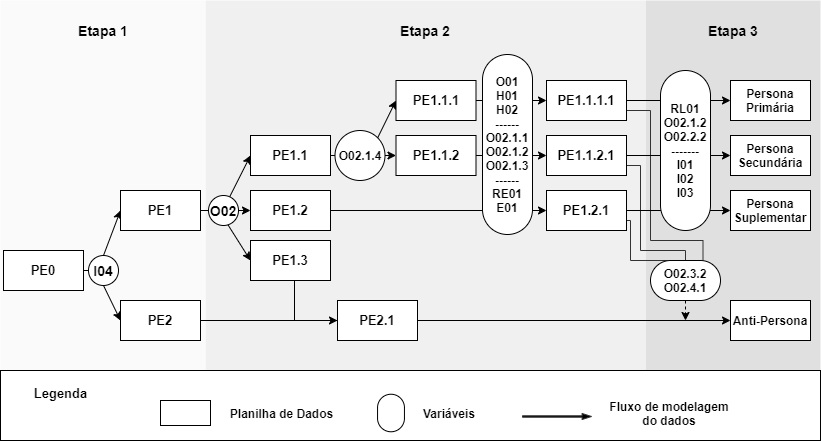
\includegraphics[keepaspectratio=true,scale=0.55]{figuras/metodologia/persona_tree.png}
	\label{Fig:persona_tree.png}
\end{figure}


A partir da variável O02 foi possível agrupar os dados em três perfis comportamentais, a partir dos dados em PE1. Foram estes, o perfil daqueles que ainda usavam jogos e os que já usaram, mas não jogavam mais (PE1.1); o perfil  daqueles que nunca jogaram, mas tinham um interesse (PE1.2); e o perfil daqueles que não tinham interesse de jogar, que no caso, este foi englobado à anti-persona.

Dentro de PE1.1 existiam aqueles que já haviam jogado, mas por algum motivo tinham parado de usar jogos para aprendizagem. Destes, foram relevantes para o objetivo do trabalho apenas os que pararam de jogar por terem alcançado seu objetivo de estudo com estes jogos. Foi obtido então PE1.1.1, com  os dados daqueles que usavam jogos para aprendizagem e PE1.1.2, aqueles que haviam jogado, mas pararam por haverem alcançado seu objetivo de estudo, que no caso foram identificados pela variável O02.1.4. Já os que usavam e deixaram de jogar e não conseguiram alcançar seu objetivo de estudo com jogos, estes foram encorporados na anti-persona.

O próximo passo foi identificar, a partir das variáveis H01 e O01, quais os perfis comportamentais seriam mais frequentes para compor personas significativas. Nesta análise, os perfis comportamentais identificados expressavam que os respondentes tinha um conhecimento sobre IHC variando entre meios formais e não formais de educação, já outros não tinham nenhum conhecimento, sendo que estes ou estavam fazendo o curso de IHC ou ainda não haviam feito.

Agrupados esses conjuntos de características foi possível definir os objetivos das personas (O02.1.1, O02.2.1 e O02.3.1). A busca por um jogo que auxilie no aprendizado de um conteúdo novo, um jogo que ajude na revisão de um conteúdo visto e um que forneça a possibilidade de avaliar o conhecimento do jogador, formando então os perfis PE1.2.1, PE1.1.1.1 e PE1.1.2.1. 

Com os objetivos das personas definidos, foram então determinadas os requisitos de jogos e as experiências (RE01 e E01, respectivamente) mais relevantes para cada um dos três perfis. Estes requisitos e experiências podem ser observadas no Apêndice \ref{ap:questionario}, nas Figuras \ref{tab:req-qualit} e \ref{tab:exp-player}, respectivamente.

Para definir a relevância de cada aspecto, foi utilizado o processo do trabalho de \citeonline{silva_sales_mendes2021} como base. A relevância de cada destes aspectos de qualidade (requisitos do jogo e as experiência do usuário) se deu pela classificação dos próprios respondentes. Estas classificações (Não é importante, Pouco importante, Indiferente, Importante e Muito importante) foram convertidas em valores numéricos inteiros, de 0 à 4, respectivamente.

Cada um dos três perfis foi caracterizado por estes aspectos de qualidade, sendo que cada um deles obteve um grau de relevância entre 0 e 664. Este grau de relevância é reflexo do somatório da pontuação que todos os respondentes (166) deram para determinado aspecto. Esses limites (0 e 664) remetem ao caso, se todos os respondentes dessem a pontuação mínima (0) para um determinado aspecto, o grau de relevância seria 0, mas se todos dessem a pontuação máxima (4), o grau de relevância seria 644.

Por exemplo, supondo que fossem 5 respondentes e dois aspectos analisados. Para o Aspecto 1 as pontuações de cada respondente respectivamente foram 3, 4, 2, 2 e 3, então o grau de relevância do Aspecto 1 seria 12, dentro do intervalo de 0 a 20. Para o Aspecto 2 as pontuações de cada respondente respectivamente foram 4, 4, 1, 3 e 2, então o grau de relevância do Aspecto 1 seria 14, dentro do intervalo de 0 a 20. Ou seja a persona que representa estes 5 respondentes teria o Aspecto 2 mais relevante que o Aspecto 1. 

Com essa estrutura base das personas, foi realizada a terceira e última fase (Figura \ref{Fig:construct_persona.png}), que visa lapidar as personas. Foi verificada a integridade das personas e se existiam redundâncias entre elas. A descrição das personas foi então detalhada, inserindo mais  atributos e comportamentos a partir das variáveis RL01, O02.1.2, O02.2.2, I01, I02 e I03. Estas serviram para dar mais realismo às personas, além de cada persona ter recebido uma foto de perfil. 

Por fim, foram designados tipos de personas: primária; secundária; suplementar e anti-persona. No caso da anti-persona, as variáveis O02.3.2 e O02.4.1 compuseram as características dela, além dos atributos considerados irrelevantes para as outras personas. O elenco de personas construídas, assim como a análise e discussão sobre os resultados se encontram descritas no Capítulo \ref{chap:result}.
